%% LaTeX2e class for student theses
%% sections/content.tex
%% 
%% Karlsruhe Institute of Technology
%% Institute for Program Structures and Data Organization
%% Chair for Software Design and Quality (SDQ)
%%
%% Dr.-Ing. Erik Burger
%% burger@kit.edu
%%
%% Version 1.3.5, 2020-06-26

\chapter{Feature generation}
\label{ch:features}
%% ==============
Neural networks and other machine learning techniques have strict requirements on their input data.
For ANNs specifically, the input needs to be of fixed size and ideally as low dimensional as possible.
In order to learn, all the data required to predict molecular properties, in this case the activation barrier, should be encoded.

Simple encoders extract well know features of molecules such as their mean electro negativity or atomic numbers \cite{LO20181538}.
Approaches by state-of-the-art chemical encoders include using graph convolutions to parse the chemical structure into fixed size features \cite{GNN_ENCODER}.
Others try to encode interaction of different atoms or species of atoms into their features \cite{PhysRevLett.108.058301}
The feature generators relevant to this project are spacial encoders.
Spacial encoders in chemistry generally focus on describing the interaction of chemical elements within a certain radius, rather 
than the space itself \cite{Bart_k_2013}.
Since global rotation translation of an element generally does not influence it's chemical properties, 
encoders try to produce rotationally invariant representations.
This however usually limits the possibilities of reconstructing the input data.
A 3D representation can therefor not easily be computed from the generated features.

The feature generators proposed here have the ability to partly reconstruct the 3D space they are encoding.
In order to retain partial rotational invariance the special stricture of the input data is used.
All catalyst molecules in the dataset have a central metal atom and a reaction pocket composed of a hydrogen atom attached to the metal center.
By the centers of these 2 atoms a unique axis is formed.
This axis is used to align the molecules.

The use of this special structure of catalyst molecules to generate partly invariant features seems to be a novel approach.

After alignment, two different approaches to feature generations are explored.
The first method slices the molecule at certain heights.
The slices are then described using a fully rotationally invariant descriptor.

The second approach is to use a combination of different 3D basis functions to encode the space surrounding the central atom.
Since this description is not fully invariant, data augmentation is used along the remaining axes of freedom.

\section{Alignment of catalyst molecules}

Every catalyst molecule $\mathbb{E}$ in the dataset has a central Iridium atom with position $p_{Ir} \in \mathbb{E}$.
We set out Iridium atom to be the center, and align all other atoms accordingly.

$$ \forall p_i \in \mathbb{E}: p_i' = p_i - p_{Ir}$$

Now that our element is centered, the next step is rotating it.
Every catalysts has a reaction pocket attached to the central metal atom.
This reaction pocket is defined by a hydrogen atom.
The goal is to rotate the entire molecule so that the reaction pocket is aligned with the $z$-Axis.
We define our axis to be aligned by the vector running from the center to the reaction pocket and normalize it, so

$$ v = \frac{p_{Pocket}'}{\| p_{Pocket}'\| } $$

The vector $v$ is now rotated so that it aligns with the $z$-Axis.
Since this rotation can be defined no matter the elements initial alignment, it effectively removes rotational invariances.
We define a plane through the points $(0,0,0), (0,0,1), v$.
The normal $n$ is the axis we will rotate the molecule around.

$$
n =\frac{\begin{pmatrix}
  0 &
  0 &
  1
\end{pmatrix}^T \times v}{ \left\| \begin{pmatrix}
  0 &
  0 &
  1
\end{pmatrix}^T \times v \right\| }
$$
Next, we define the angle $\alpha$ between $v$ and the $z$-Axis on the plane.

$$ 
\alpha = k \cdot \arctantwo \left( 1,  
\begin{pmatrix} 0 &  0 & 1 \end{pmatrix} \cdot v \right),\space k = \left\{\begin{array}{ll} 1, & n \cdot \left( (0,0,1)^T \times v \right) > 0 \\
  -1, & \text{otherwise}\end{array}\right.
$$

This gives a rotation matrix around the normal.
$$
R(\alpha) = I_3 + C \sin(\alpha) + C^2(1 - \cos(\alpha)), C =
\begin{pmatrix}
  0 & -q_0 & q_1 \\
  q_2 & 0 & -q_0\\
  -q_1 & q_0 & 0
\end{pmatrix}
$$


The rotation $R(\alpha)$ can then be applied to all centered atom.
The aligned and centered molecule can therefor be described as

$$ 
\mathbb{E}^R = \left\{ R(\alpha) (p_i - p_{Ir}) |  p_i \in \mathbb{E} \right\}
$$

The coordinates $p^R_i \in \mathbb{E}^R$ are now rotationally invariant under 2 axes. 
The only degree of freedom left is rotations around the vector $v$. 

We will repeat this normalization for every element in the dataset.

Since there's no natural way to align the elements around $v$, different approaches will be used.
In a first attempt, features are generated using a descriptor that is invariant under rotations around $v$.
The second descriptor is using data augmentation to teach the network about possible rotations of the molecule.

\section{Fourier descriptors for invariant feature generation}

The first attempt at feature generation was using a fully rotational invariant feature descriptor.
The method used is an Elliptic Fourier Descriptor (EFD).
Elliptic fourier descriptors approximate a 2D contour with a set of coefficients.
The higher the order of the descriptor, the better a contour can be approximated.

To be able to describe a 3D object using fourier contour descriptors the object is sliced at different $z$ locations.
These slices can then be described using an EFD.

\subsubsection{Slicing}

\begin{figure} [h]
  \centering
  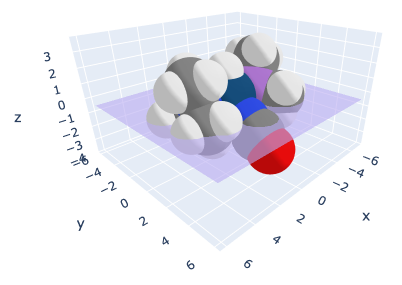
\includegraphics[width=0.5\textwidth]{figures/fourier/slice3d.png} % for .pdf files etc use \includegraphics{test.pdf}
  \caption{A molecule is sliced by a plane. Every slice is taken at a different $z$ height.}
  \label{fig:slice3d}
\end{figure}

Along the $z$-axis, starting from $z_{start}$ to $z_{end}$, the molecule is sliced in a distance of $z_{height}$.
$z_{start}, z_{end}, z_{height}$ are tuning parameters.
Here, $z_{start}, z_{end}$ are chosen so that all molecules from the dataset fully fit into the boundaries.

A slice is computed by getting the radius of every atom $i$ in the molecule at the slice height $z$ \ref{fig:slice3d}.

$$ r_i(z) =\left\{\begin{array}{ll} \sqrt{R_i^2 - (z - p_i^R[2])^2} &, | z - p_i^R[2] |  < R_i\\
  0 &, \text{otherwise}\end{array}\right.
$$ %TODO: Der Betrag ist immer > 0 ???

Here $R_i$ is the Van-der-Waals radius of element $i$, $p_i[2]$ is the $z$ component of the location vector.
The slice is now constructed by drawing a circle with radius $r_i(z)$ around the $x,y$ coordinates for each atom for each slice Figure~\ref{fig:slice}.

\begin{figure} [h]
  \centering
  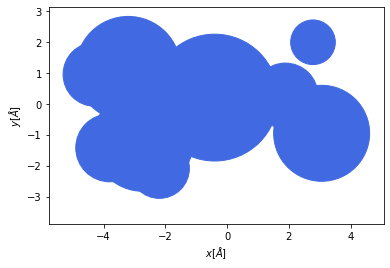
\includegraphics[width=0.5\textwidth]{figures/fourier/slice-iso.png} % for .pdf files etc use \includegraphics{test.pdf}
  \caption{A slice with isolates.}
  \label{fig:slice}
\end{figure}

The slice now consists of a set of circles.
These circles can be partially or fully intersecting. 

To describe the contour, a fourier contour descriptor is used.
This contour descriptor allows to easily ignore rotation of the contour and generate invariant low-dimensional features from the shape.
However, it can only work on a closed contour, so isolate islands of circles that don't intersect have to be dealt with separately.

To identify islands and one continuos subset of circles, for each slice a graph is constructed.
For every atom with radius $>0$ we create a node.
For every atom that intersects with another we create an edge between these two nodes.
Now the \texttt{Largest Connected Component}, so the connected subgraph with the most nodes, is selected.
This gives us the most atoms forming a continuously connected shape in the current slice.
In the next steps we will only only use this subset to describe the contour.

\paragraph{Finding the contour}

From the set of intersection circles, the contour needs to be extracted. 
Since the contour points need to be computed just from radius and position information, and are not rendered onto a 2D pixel grid, standard contour finding algorithms can not be used.
Instead, knoledge about the general shape is used to compute the contour. 

The contour is computed using \autoref{alg:CircleSetContour}.

First, the point "furthest to the right", so with the largest x-Value is found. 
Since the point with the highest x-Value in any circle is always at angle 0, we set the intial angle $\alpha$ and rotation vector $\vec{p}$ accordingly.
From the circle containing that point, the contour is followed from that point counter-clockwise until the first intersection with another cirlce is found \autoref{fig:contour1}.
To the list of countour sections, we add the current contour section from angle 0 to the angle of intersection.

Now, the contour of this circle is followed again until it intersects another. This is reapeated until the starting circle is reached again \autoref{fig:contour2}.

Once the starting circle is reached, the last remaing contour part of the starting circle needs to be added to the list of contour sections \autoref{fig:contour3}.

From the ordered list of contour sections, the contour points can easily be computed.
Since each contour section consits of a radius $r$, location $(x,y)$, and start- and end angle $\alpha_{start}, \alpha_{end}$, the coordinates of the contour points can simply be computed using $x_c = \cos(\alpha_c) \cdot r + x$ and  $y_c = \sin(\alpha_c) \cdot r + y$ 
for $\alpha_c = \alpha_{start} + i \cdot \Delta, \alpha_c \leq \alpha_{end}$.
$\Delta$ is a tuning paramter that specifies the resolution of the contour.

This process of going along the outside ignores all "holes" in the shape, so only the outermost contour will be part of the final result. 

\begin{figure}[!htb]
  \minipage{0.32\textwidth}
    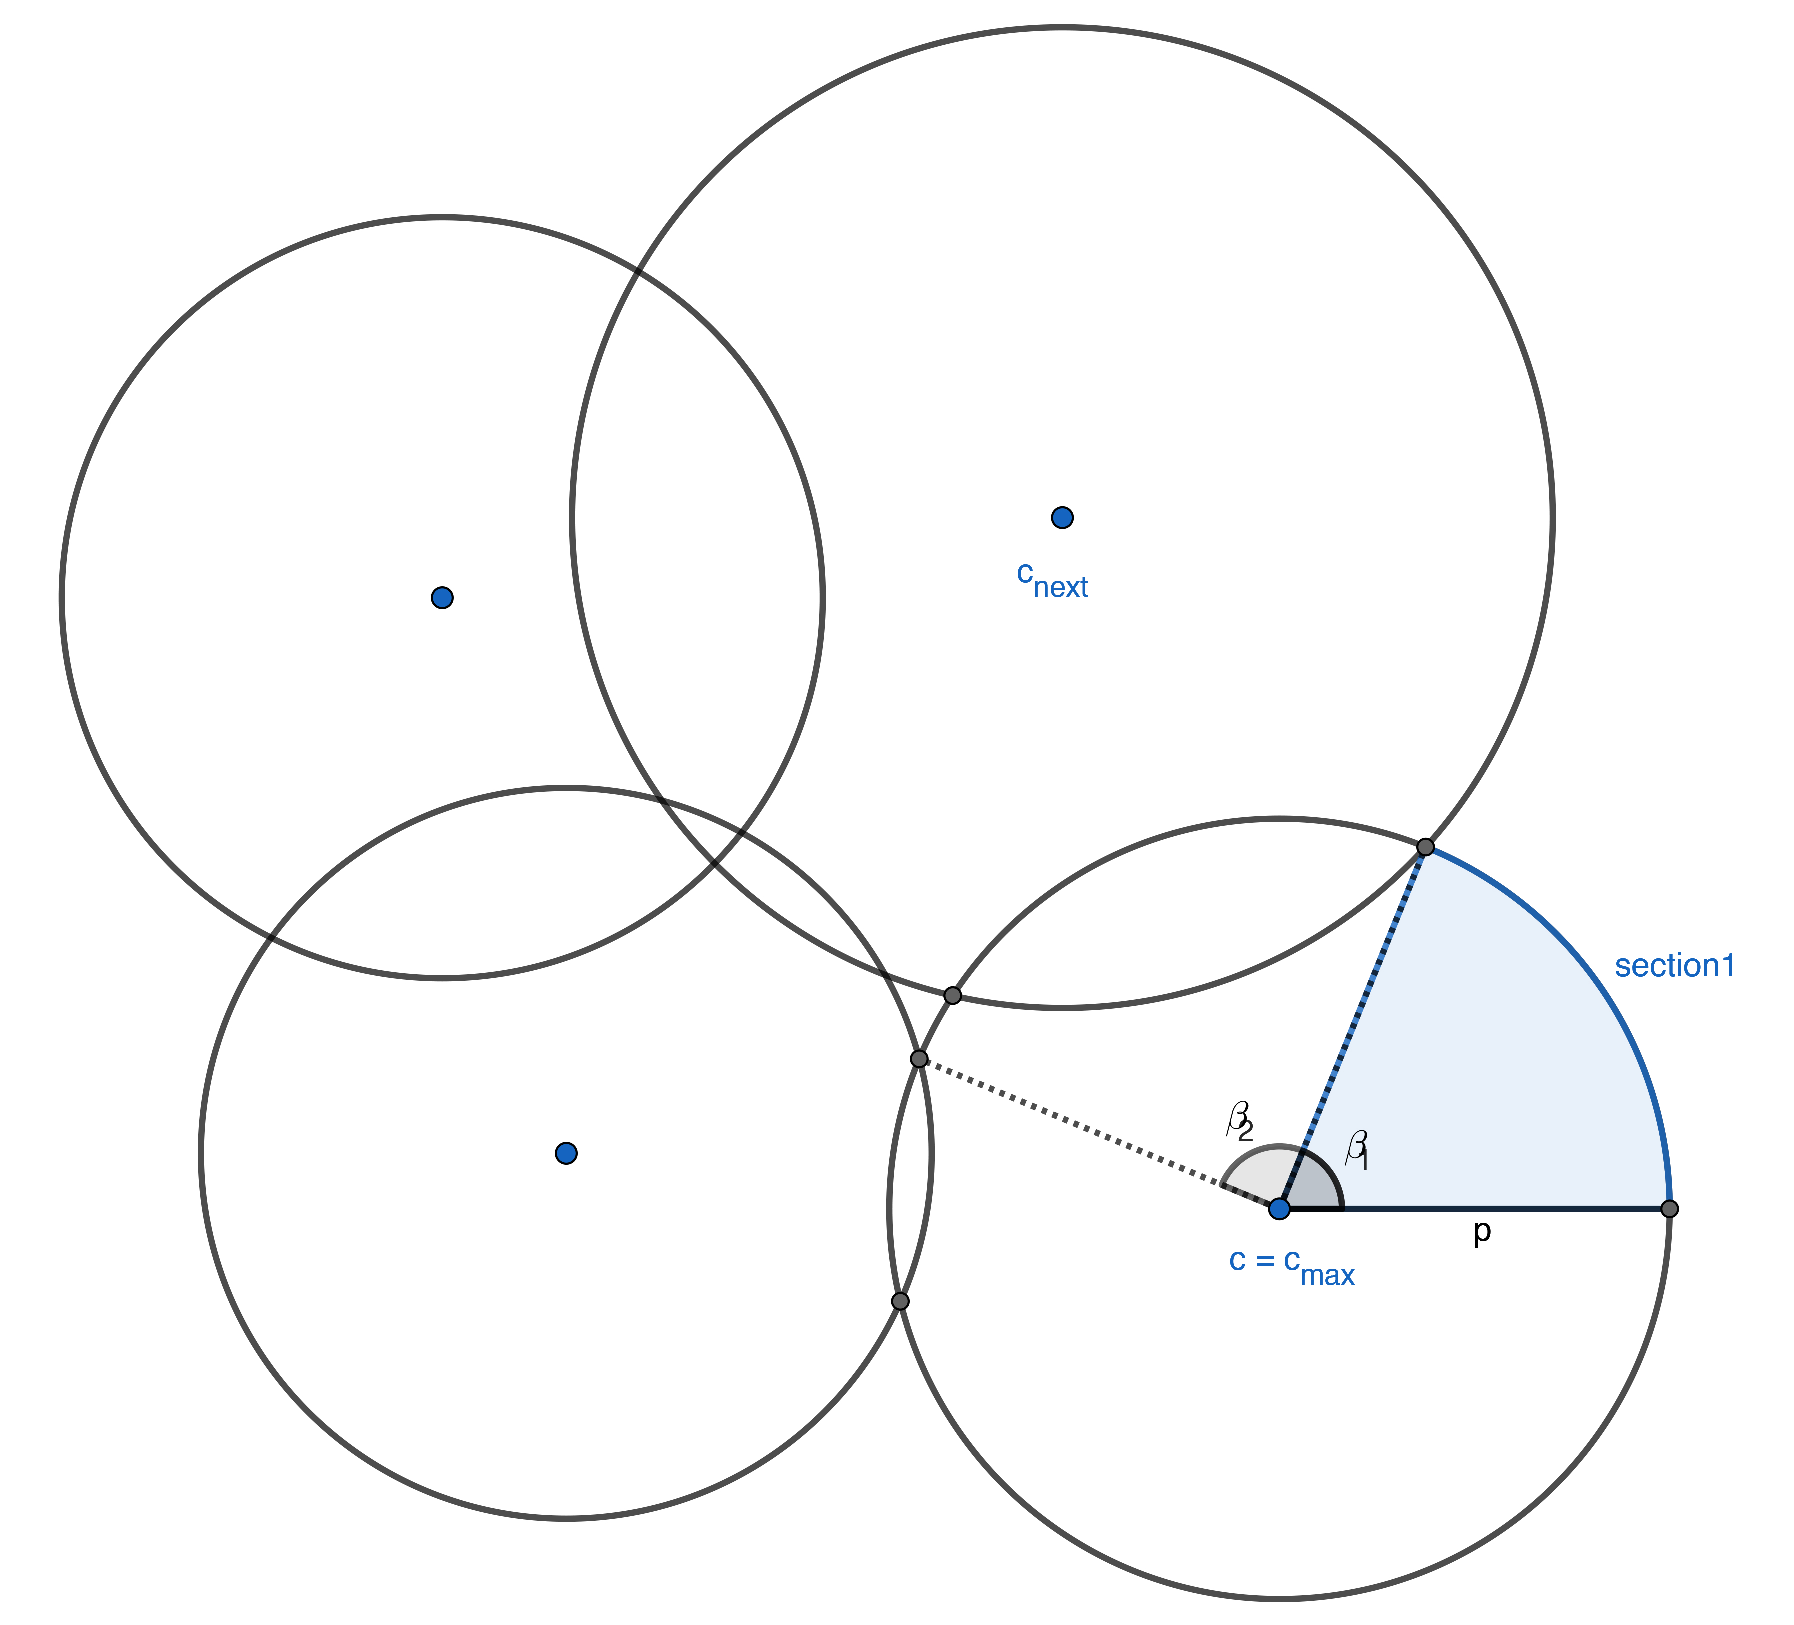
\includegraphics[width=1.0\textwidth]{figures/contour/c1copy.pdf}
    \caption{Finding first contour section}\label{fig:contour1}
  \endminipage\hfill
  \minipage{0.32\textwidth}
    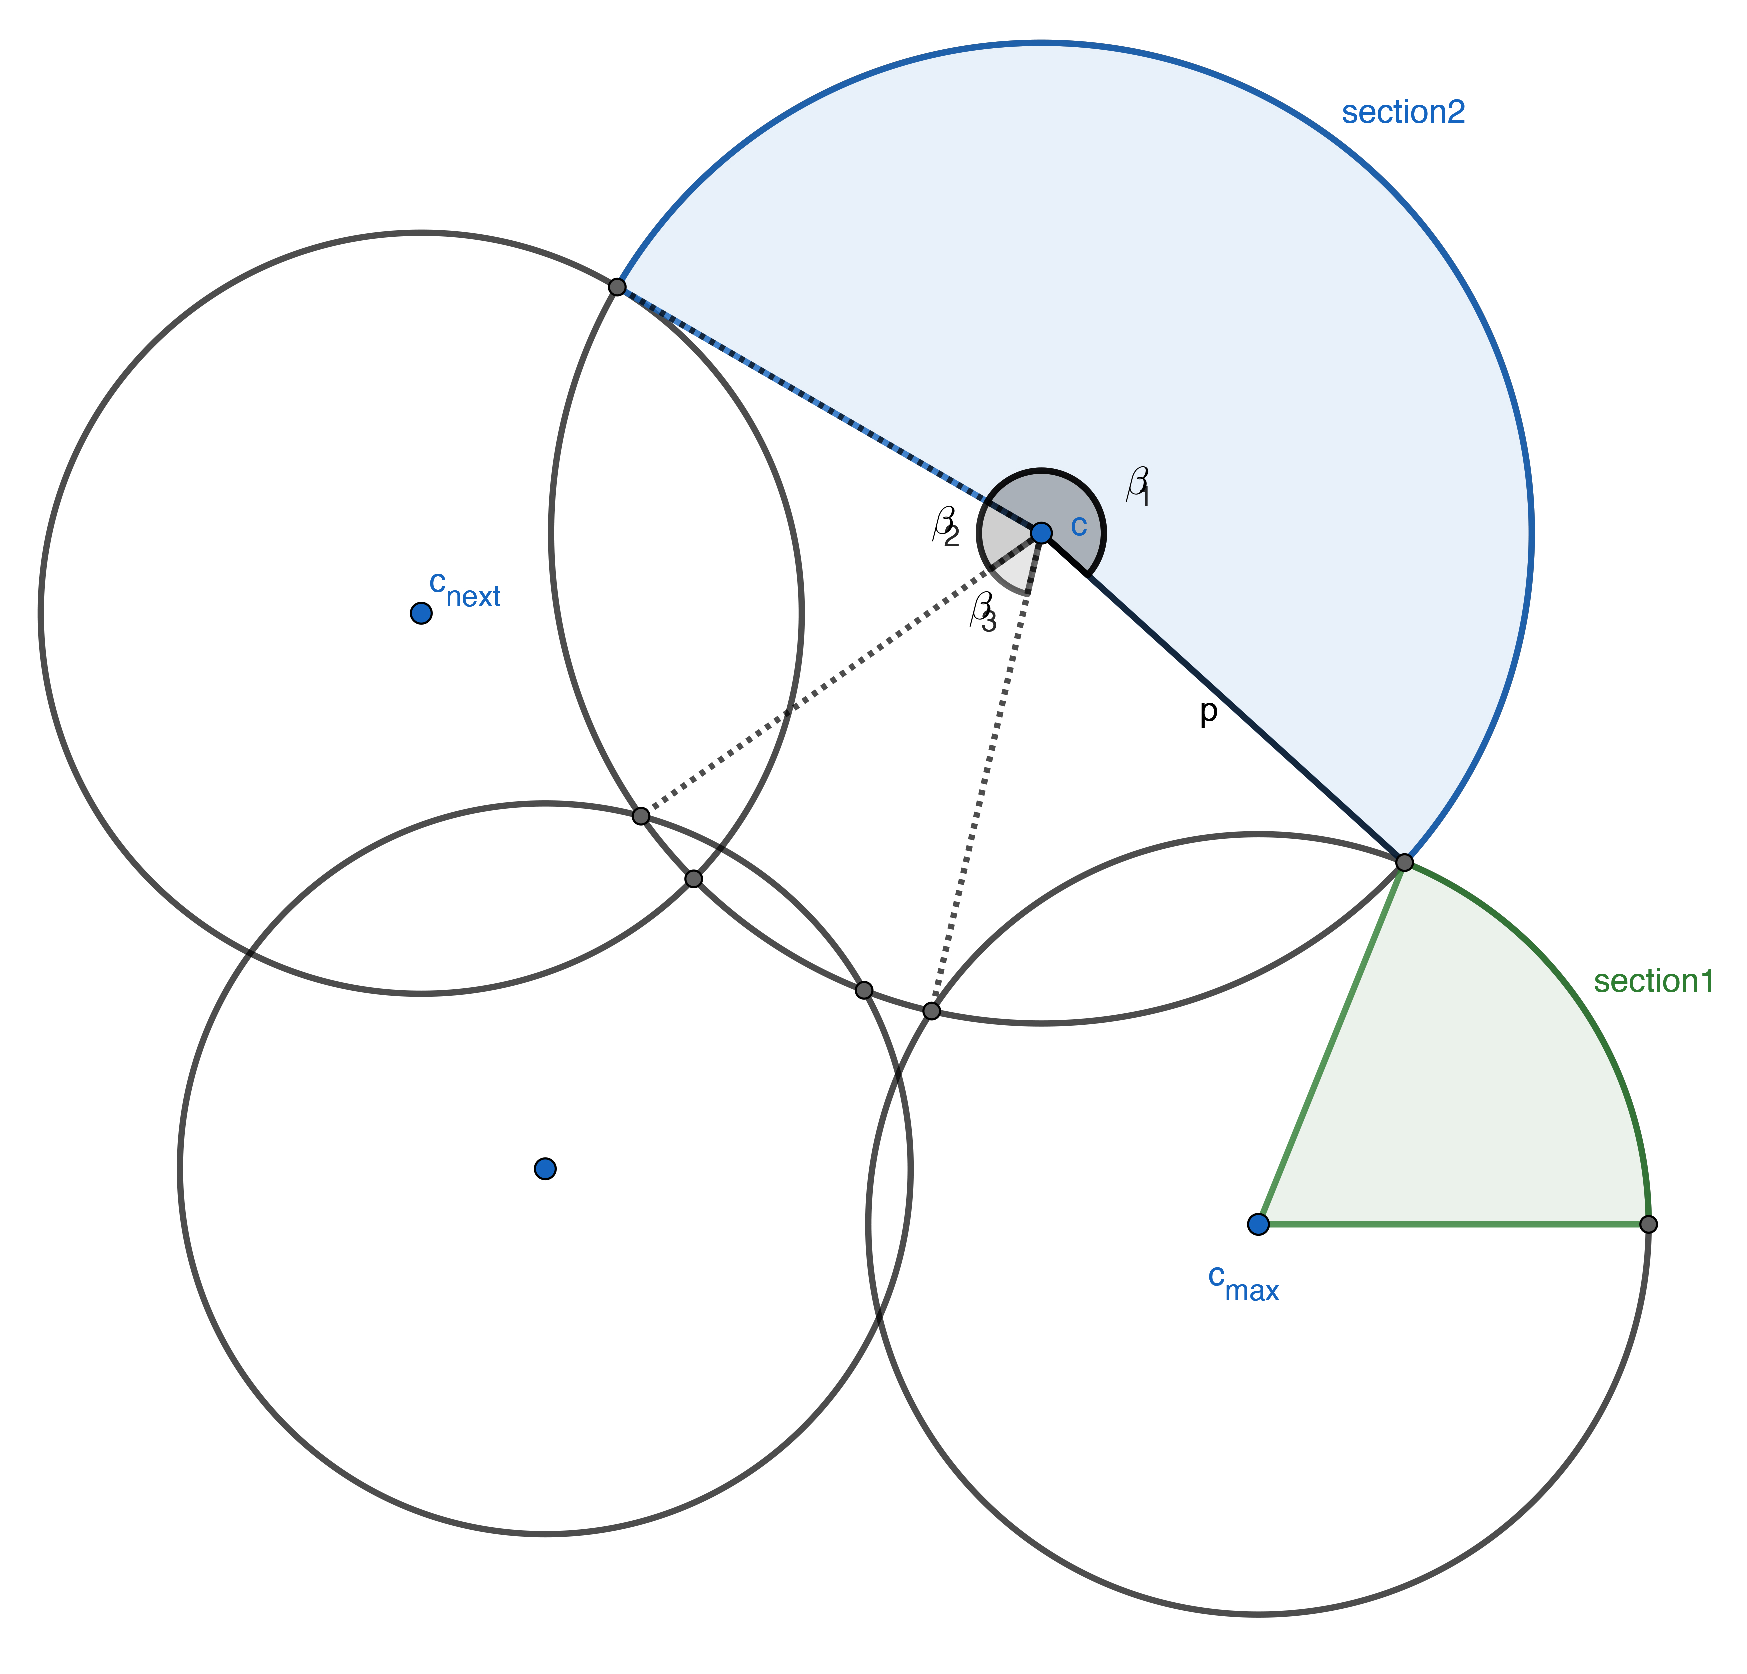
\includegraphics[width=1.0\textwidth]{figures/contour/c2copy.pdf}
    \caption{Finding middle contour section}\label{fig:contour2}
  \endminipage\hfill
  \minipage{0.32\textwidth}%
    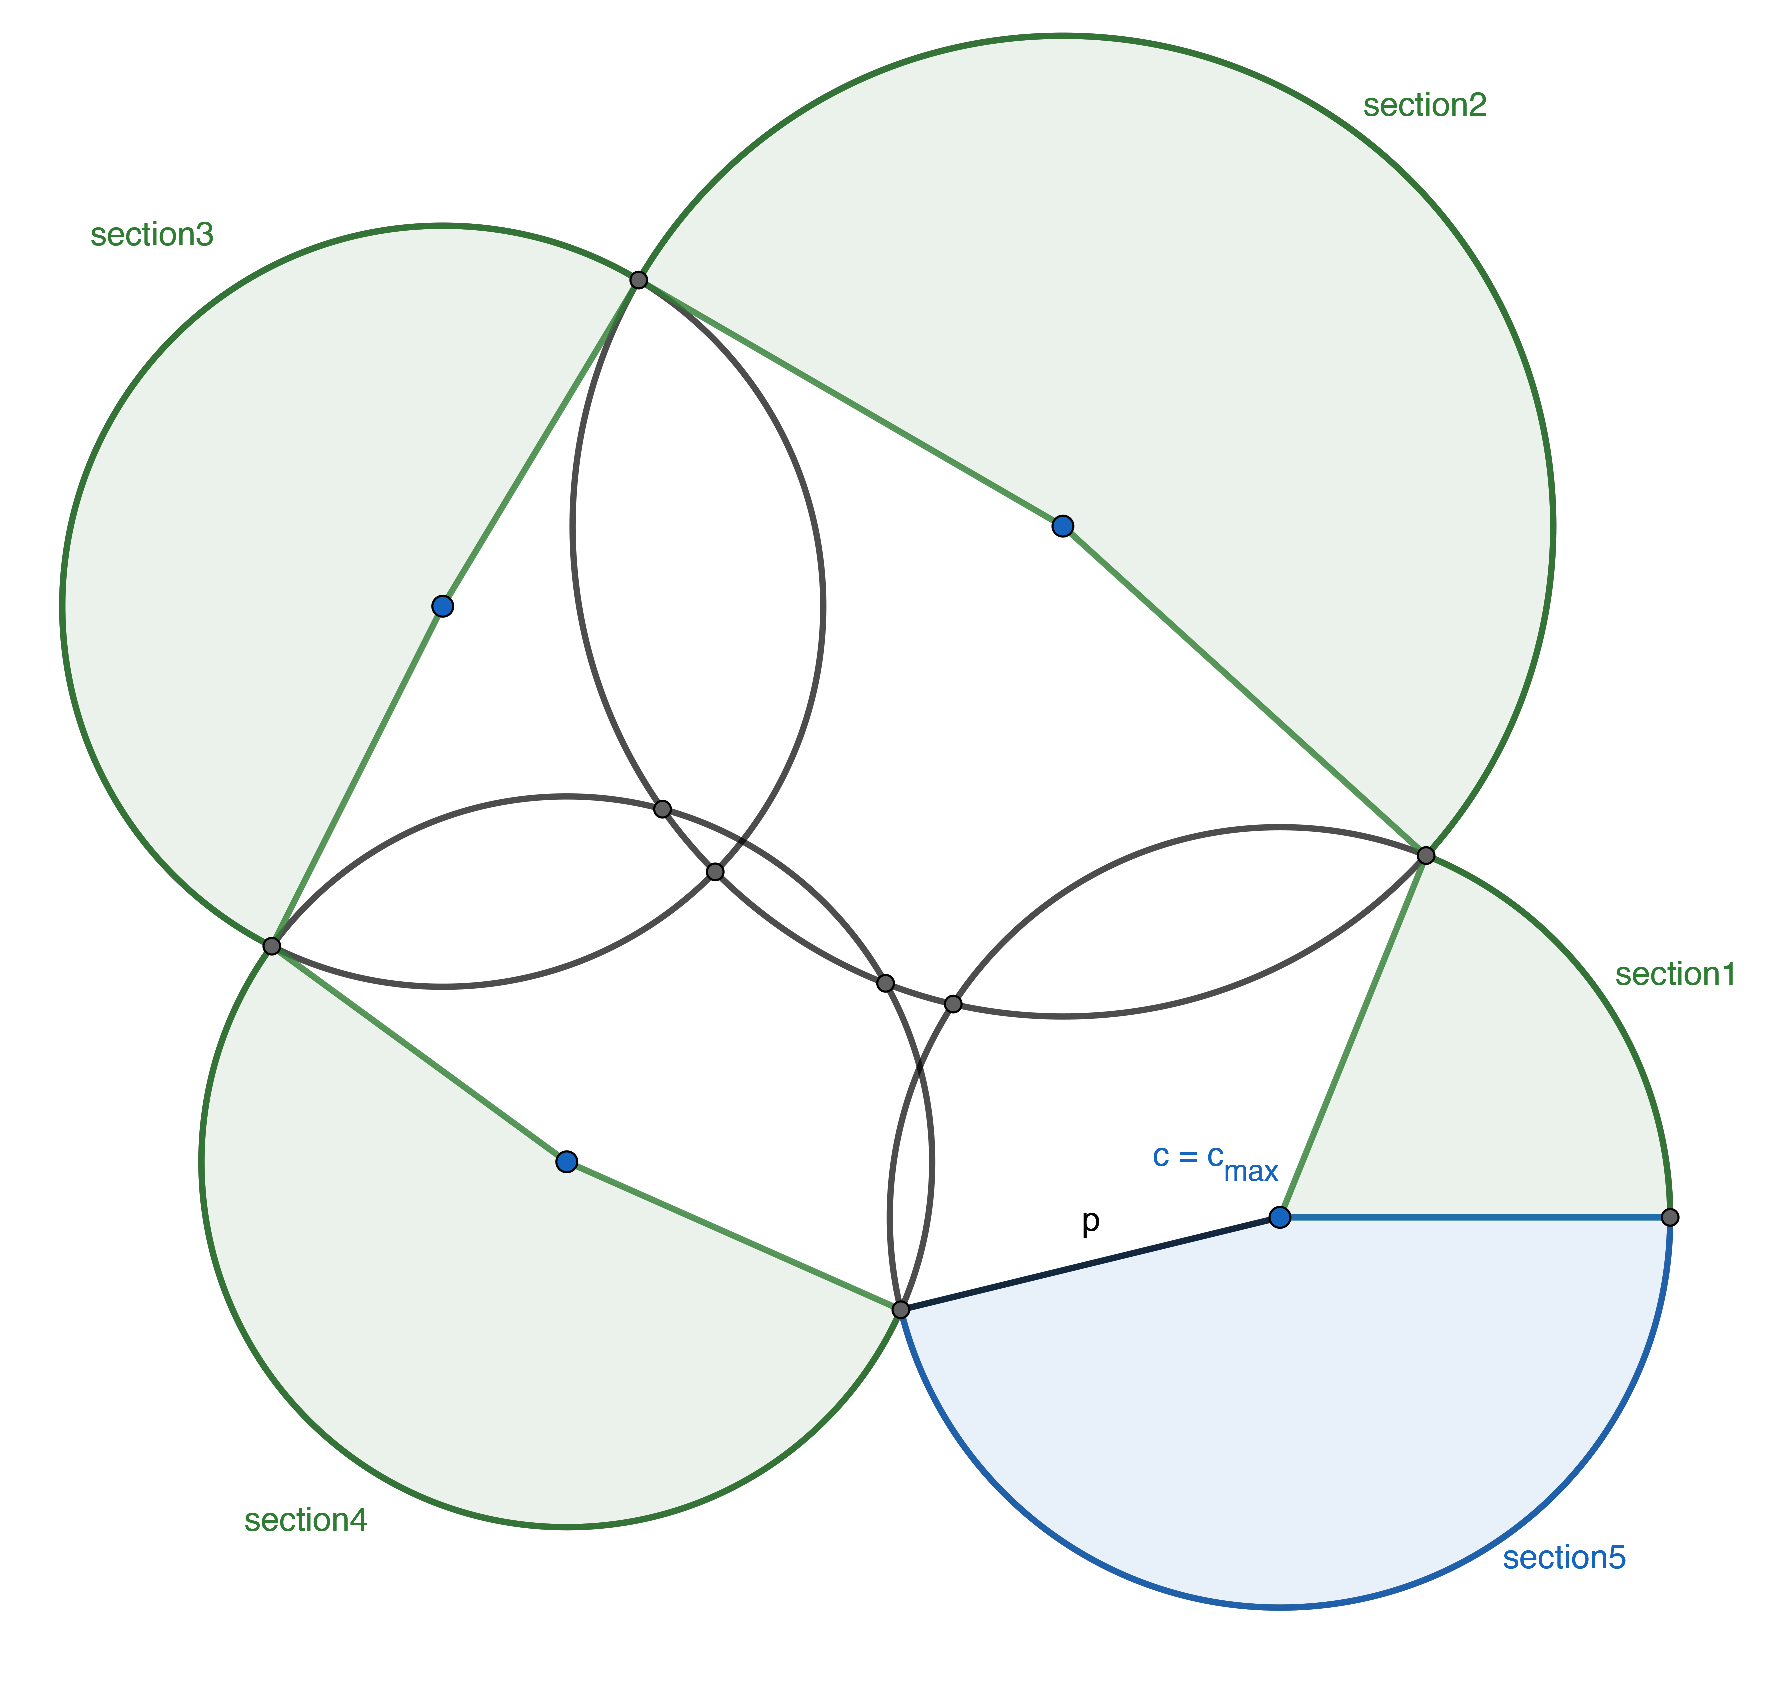
\includegraphics[width=1.0\textwidth]{figures/contour/c3copy.pdf}
    \caption{Finding the last contour section}\label{fig:contour3}
  \endminipage
\end{figure}


\paragraph{Eliptic fourier descriptor}

Now that we have a contour for each slice, we'll use the elliptic fourier descriptor (EFD) to describe that contour.
The advantages of EFDs is that they allow to encode contours with relatively few coefficients. 
Additionally, EFD coefficients can easily be made rotationally invariant.

EFDs, as described in \cite{LIN1987535} work by selecting a random starting point $s$ on the contour.
Starting from $s$, we will follow the contour and denote the $x$ and $y$ coordinates as functions $x(l)$, $y(l)$ of the distance $l$ from the starting point.
Distance refers to the length it takes to get from $s$ to the point following the contour.

Since the starting and end point of $x(l), y(l)$ will be equal, making them periodic, we can define a parameter $t=\frac{2\pi l}{n}$.
The functions can then be described by Fourier expansions as

%TODO: Replace t and put it in directly?
$$
\begin{pmatrix}
  x(l) \\
  y(l) \\
\end{pmatrix}
=
\begin{pmatrix}
  a_0 \\
  d_0 \\
\end{pmatrix}
+
\sum_{k=1}^\infty 
\begin{pmatrix}
  a_k & b_k\\
  c_k & d_k\\
\end{pmatrix}
\cdot
\begin{pmatrix}
  \cos(kt)\\
  \sin(kt)\\
\end{pmatrix}
$$

with

$$
a_0 = \frac{1}{2\pi} \int_{0}^{2 \pi}  x(t) \,dt 
$$
$$
d_0 = \frac{1}{2\pi} \int_{0}^{2 \pi}  y(t) \,dt 
$$

$$
a_k = \frac{1}{\pi} \int_{0}^{2 \pi}  x(t) \cos(kt) \,dt 
$$
$$
b_k = \frac{1}{\pi} \int_{0}^{2 \pi}  x(t) \sin(kt) \,dt 
$$
$$
c_k = \frac{1}{\pi} \int_{0}^{2 \pi}  y(t) \cos(kt) \,dt 
$$
$$
d_k = \frac{1}{\pi} \int_{0}^{2 \pi}  y(t) \sin(kt )\,dt 
$$

The $a_k, b_k, c_k, d_k$ form a basis for the functions $x(l), y(l)$.
By addition of the vector $ \begin{pmatrix} a_0 & b_0 \end{pmatrix}^T $ an offset can be defined.
Since the contours encoded here should stay rotationally invariant, a two dimensional offset is not feasible.
Instead, we will add the offset length $\|  \begin{pmatrix} a_0 & b_0 \end{pmatrix}^T \| $ as part of the feature vector.

The last step is making the fourier descriptor rotationally invariant.
So far, the features $a_k, b_k, c_k, d_k$ are depended on the rotation of the contour.
The next step will be to make te features invariant under rotations.
%%%The starting point $s$ does not affect the coefficients as shown by \citeauthor{KUHL1982236}.

We can view the contour as a summation of ellipses of different size.
By aligning the first ellipse and rotating all other ellipses accordingly, we can make the final output invariant
of rotation \cite{MEBA}.

$$
\theta = \frac{1}{2}\arctan \left( \frac{2(a_1b_1 + c_1d_1)}{a_1^2 + c_1^2 - b_1^2 - d_1^2} \right)
$$
$$
\psi = \arctan \left( \frac{\cos(\theta) a_1 + \sin(\theta) b_1 }{\cos(\theta) c_1 + \sin(\theta) d_1} \right)
$$

The aligned coefficients $a_k^R, b_k^R, c_k^R, d_k^R$ can then be obtained using

$$
\begin{pmatrix}
  a_k^* & b_k^* \\
  c_k^* & d_k^* \\
\end{pmatrix}
=
\begin{pmatrix}
  \cos(\psi) & -\sin(\psi) \\
  \sin(\psi) & \cos(\psi) \\
\end{pmatrix}
\begin{pmatrix}
  a_k & b_k \\
  c_k & d_k \\
\end{pmatrix}
\begin{pmatrix}
  \cos(k\theta ) & -\sin(k\theta) \\
  \sin(k\theta) & \cos(k\theta) \\
\end{pmatrix}
$$.

The rotation around $\theta $ can be interpreted as normalizing the starting point $v$, 
the rotation around $\psi$ as normalizing the rotation of the contour itself \cite{KUHL1982236}.

The last step is to choose an order up to witch we want to approximate the contour.
At the moment the infinite sum ensures a perfect approximation original contour. 
By limiting the coefficients to an order $k_{max}$ we can set the number of coefficients describing our contour.
Generally, the higher we choose our order, the better we can approximate small changes in the contour \ref{fig:slice-layered}.

After normalizing, the values $b_1^* = c_1^* = 1$ will always be equal to 0, since we rotated the first ellipse to be aligned.
We can therefore remove $b_1^*, c_1^*$ from the feature vector.

After calculating the coefficients for every slice, the different slices will be concatenated into a 2d array.
One dimension of the array will correspond to the spacial $z$ direction, so it will be equivalent to the number of layers we choose.
The other dimension will hold the fourier coefficients for each layer.
To keep information about the offset from the center, the length $l = \| \begin{pmatrix} a_0 & b_0 \end{pmatrix} \| $ will be added for each slice.
Since each fourier coefficient consists of 4 values and we remove $b_1^*, c_1^*$ and add the center offset $l$, the size of this dimension will be $k_{max} * 4 - 1$.

These features will be used for predictions of molecule in the next step.

\begin{figure}[!htb]
  \minipage{0.4\textwidth}
    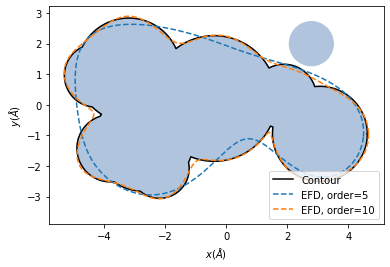
\includegraphics[width=1.0\textwidth]{figures/fourier/contour.png}
  \endminipage\hfill
  \minipage{0.6\textwidth}
    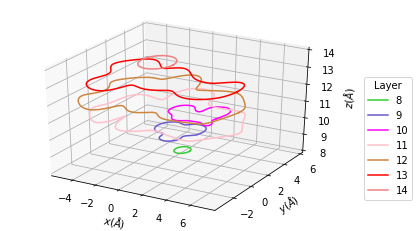
\includegraphics[width=1.0\textwidth]{figures/fourier/fourier-slices.png}
  \endminipage
  \caption{
  On the left a slice is described by fourier descriptors. Higher order descriptors are able to approximate the contour better than lower order descriptors. 
  The isolate is ignored by the contour descriptor. The rotation is kept as part of the fourier description for illustration purposes.
  On the right the different slices making up on element are placed on top of each other. Slices without any volume are not rendered. 
  Wile the rotation is removed to keep it rotationally invariant, the offset from the center is encoded.
  }
  \label{fig:slice-layered}
\end{figure}

\section{Feature generation using smooth normalized atomic positions}

In a second approach, the molecule was encoded using by smoothing the atomic positions, 
and then combining a set of functions describing the 3D space around the metal center.

This method is partly similar to the Smooth Overlap of Atomic Positions (SOAP) descriptor, that produces a 
fully rotational invariant description for the space surrounding one or more atomic centers \cite{Bart_k_2013}.
Specifically the gaussian smoothing of atomic positions and combination of radial basis functions with
spherical harmonics to describe a 3D space is taken from SOAP.
While SOAP describes the overlap of densities for different species, the goal here is to describe the density space directly.
The disadvantage of SOAP is that due to the rotational invariance, the 3D environment cannot be reconstructed from the generated features.

The Smooth Normalized Atomic Positions (SNAP) descriptor proposed here allows for a reconstruction of the 3D space from the coefficients, 
while partly keeping the rotational invariance.
Rotational invariance however is not given by the feature generation itself, but rather by using the catalysts special struture.
The SNAP descriptor therefor is less universal than SOAP. 
In applications were no translation back to 3d space is required,
in most instances SOAP should be chosen for it's fully rotationally invariant output.

\subsection{SNAP requirements}

The general idea of SNAP is to describe the density surrounding a cental atom using a fixed set of coefficients.
Rotational invariance therefore cannot be guaranteed, unless the encoded molecule itself can be rotated in a way to explicitly set it's rotation.

For catalyst molecules, this natural axis can be defined by setting the reaction pocket to the top, and the central Iridium atom as a center.

For other molecule classes, defining a natural axis might not be as trivial.

When no clear axis of alignment can be found, the SNAP output may be augmented by rotating the input along all axis of freedom.
If there are multiple axis of freedom SOAP may be preferable since in naturally offers a fully rotationally invariant description.

Additionally, SNAP only encodes a local region within $r_{cut}$.
Density outside this cutoff radius is not considered.
Is a global description of the entire element is needed, SNAP might not be the best option, especially when 
the size of the elements in the dataset varies a lot.


\subsection{SNAP}

Using the centered and aligned molecules, we will create the density space surrounding out central atom.

By generating 3D gaussian distributions for every atom in the element, we can calculate the density at any point within $r_{cut}$.
For each species $Z$ in the dataset, the density at any point $p = (x,y,z)$ is described as

$$\rho^Z(p) = \sum_i^{|Z|} e^{- \frac{1}{2\sigma^2} \vert p - R_i \vert^2 }$$ 

The summation $i$ runs over all the atmos of that species. $R_i$ is the center of that atom.
In further enhancements of the SNAP encoder, describing other molecular properties in the same way are thinkable.
Even describing 3D features not associated with a single species but rather describing the interaction or overlap of species 
or molecules are thinkable.

Since the basis set we're using to describe the space is using spherical coordinates, from now on
cartesian coordinated will be replaced by spherical coordinates.

$$
r = \sqrt{x^2 + y^2 + z^2}
,
\theta = \arccos(\frac{z}{r})
,
\varphi = \arctan(y / x)
$$

The density space can then be expanded using a combination of basis functions.
To expand the radial degrees of freedom, spherical harmonics are used.
Spherical harmonics are a complete set of orthonormal basis functions describing the surface of a sphere.
We use the Laplacian Spherical Harmonicas, defined as:
$$
Y_{lm}(\theta, \varphi) = (-1)^m \sqrt{\frac{2l + 1}{4 \pi} \frac{(l - m)!}{(l + m)!}} P_{lm}\left(\cos(\theta) \right) e^{im\theta}
$$
%TODO: Add plot of first n spherical harmonics



Here, $P_{lm}$ are the associated Legendre polynomials, defined as

$$
P_{lm}(x) = (-1)^m (1-x^2)^{m/2} \frac{\partial^{l+m}}{\partial x^{l+m}}(x^2 - 1)^l
$$ %TODO: Looks at derivative


This gives us a way to encode a sphere around our central atom. 

\begin{figure} [h]
  \centering
  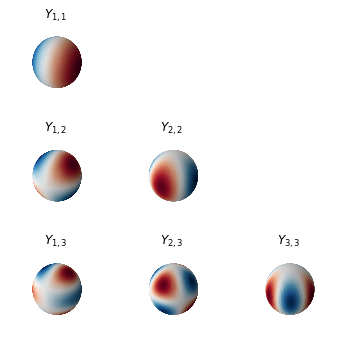
\includegraphics[width=0.5\textwidth]{figures/snap/sph-harm.png} % for .pdf files etc use \includegraphics{test.pdf}
  \caption{A selection of low order spherical harmonics plotted on a sphere. } %TODO: Add scale!!!
  \label{fig:sphharm}
\end{figure}

To encode density information along the radial direction, we combine spherical harmonics with radial basis functions.
A variety of radial functions can be used for this application.
In \cite{KUHL1982236} the use of polynomial radial function is suggested.
However here a set of primitive gaussian type orbitals are used.
This set allows for analytical integration which allows for a significant speedup over numerical integration since it can be precomputed.  
These gaussian type orbitals are defined as

$$g_{nl}(r) = \sum_{n'}{n_{max}} \beta_{nn'l} \phi_{n'lr}(r) $$

with 

$$\phi_{nl}(r) = r^l e^{-\alpha_{nl}r^2} $$ %TODO: phi of n oder phi of nl?? / alpha_n oder alpha_nl


\begin{figure} [h]
  \centering
  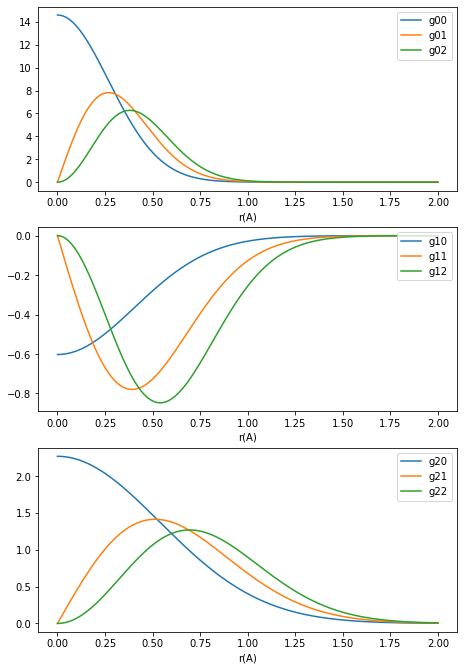
\includegraphics[width=0.5\textwidth]{figures/snap/gaus_orb.png} % for .pdf files etc use \includegraphics{test.pdf}
  \caption{Spherical gaussian orbital functions for a cutoff radius $r_{cut}=2$, $2$, $n_{max}=2$ and $l_{max}=2$. }
  \label{fig:gaussians}
\end{figure}

$\alpha$ and $\beta$ are constants that only need to be computed once for every pair of $l,m, r_{cut}$.
$\alpha_{nl}$ is a set of decay parameters chosen so that each non orthonormalized function $\phi_{nl}$ 
will decay to a threshold value of $10^{-3}$ at the cutoff radius $r_{cut}$.
%TODO: What does the 10^-3 mean?

The weights $\beta_{nn'l}$ are chosen so that the radial basis functions are orthonormal.
For each $l$ the weights $\beta_{nn'l}$ can be computed using the Löwdin orthonormalization:

$$\beta = S(l)^{-1/2} $$

with the entries of the matrix $S$ being defined as

$$S(l)_{nn'} = \langle \phi_{nl} | \phi_{n'l} \rangle  $$

The implementation of $\alpha$ and $\beta$ prefactors is taken from \cite{dscribe} where they are precomputed up to $l \leq 9$.
Higher order factors could be added if needed.


Combining spherical harmonics with radial basis functions we can describe the density space surrounding our central atom.
In theory, choosing infinitely high $n, l$ we could approximate the space with infinitely high precision.
To get a fixed amount of coefficients, $n_{max}$ and $l_{max}$ need to be chosen that determine the
accuracy of the encoding.
Generally, the higher we choose $l, m$ the more accurate we can approximate the space.
%TODO Add figure of the space being described with different n, l , cutoff

For radial basis functions we need to define a cutoff radius $r_{cut}$.
Densities outside this cutoff radius will not be encoded in the features of our space.

The density for every species $Z$ in within the cutoff sphere can be expanded as:

$$ \rho^Z(r) = \sum_{nlm} c^Z_{nlm} g_{nl}(r) Y_{lm}(\theta, \varphi) $$

The coefficients $c_{nlm}^Z$ are features generated by the SNAP descriptor.

$$ c_{nlm}^Z = \iiint_{R^3} g_{nl}(r) Y_{lm}(\theta, \varphi) \rho^Z(r, \theta, \phi)  \,dr\theta\phi   $$
% TODO: Integrate to infinity or r_cut?

The 3 dimensional integral goes over all spherical coordinates within our cutoff sphere.
The coefficients $c_{nlm}$ now describe the 3d space within a fixed size sphere.
\\
The key difference between SNAP and other chemical descriptors is the bi-directional mapping between feature space and 
density space.
From the coefficients, the density space encoded can be easily reconstructed.
This allows for a partial reconstruction of the molecule from the features encoded by SNAP.

However, due to the low number of radial basis functions and spherical harmonics usually used to describe an element, 
the encoding of the density is far from perfect.
While with an infinite amount of coefficients an perfect description of the space is thinkable,
in reality the computational limits only allow for a rather low resolution of the density space \ref{fig:snap-density}. 
\begin{figure} [h]
  \centering
  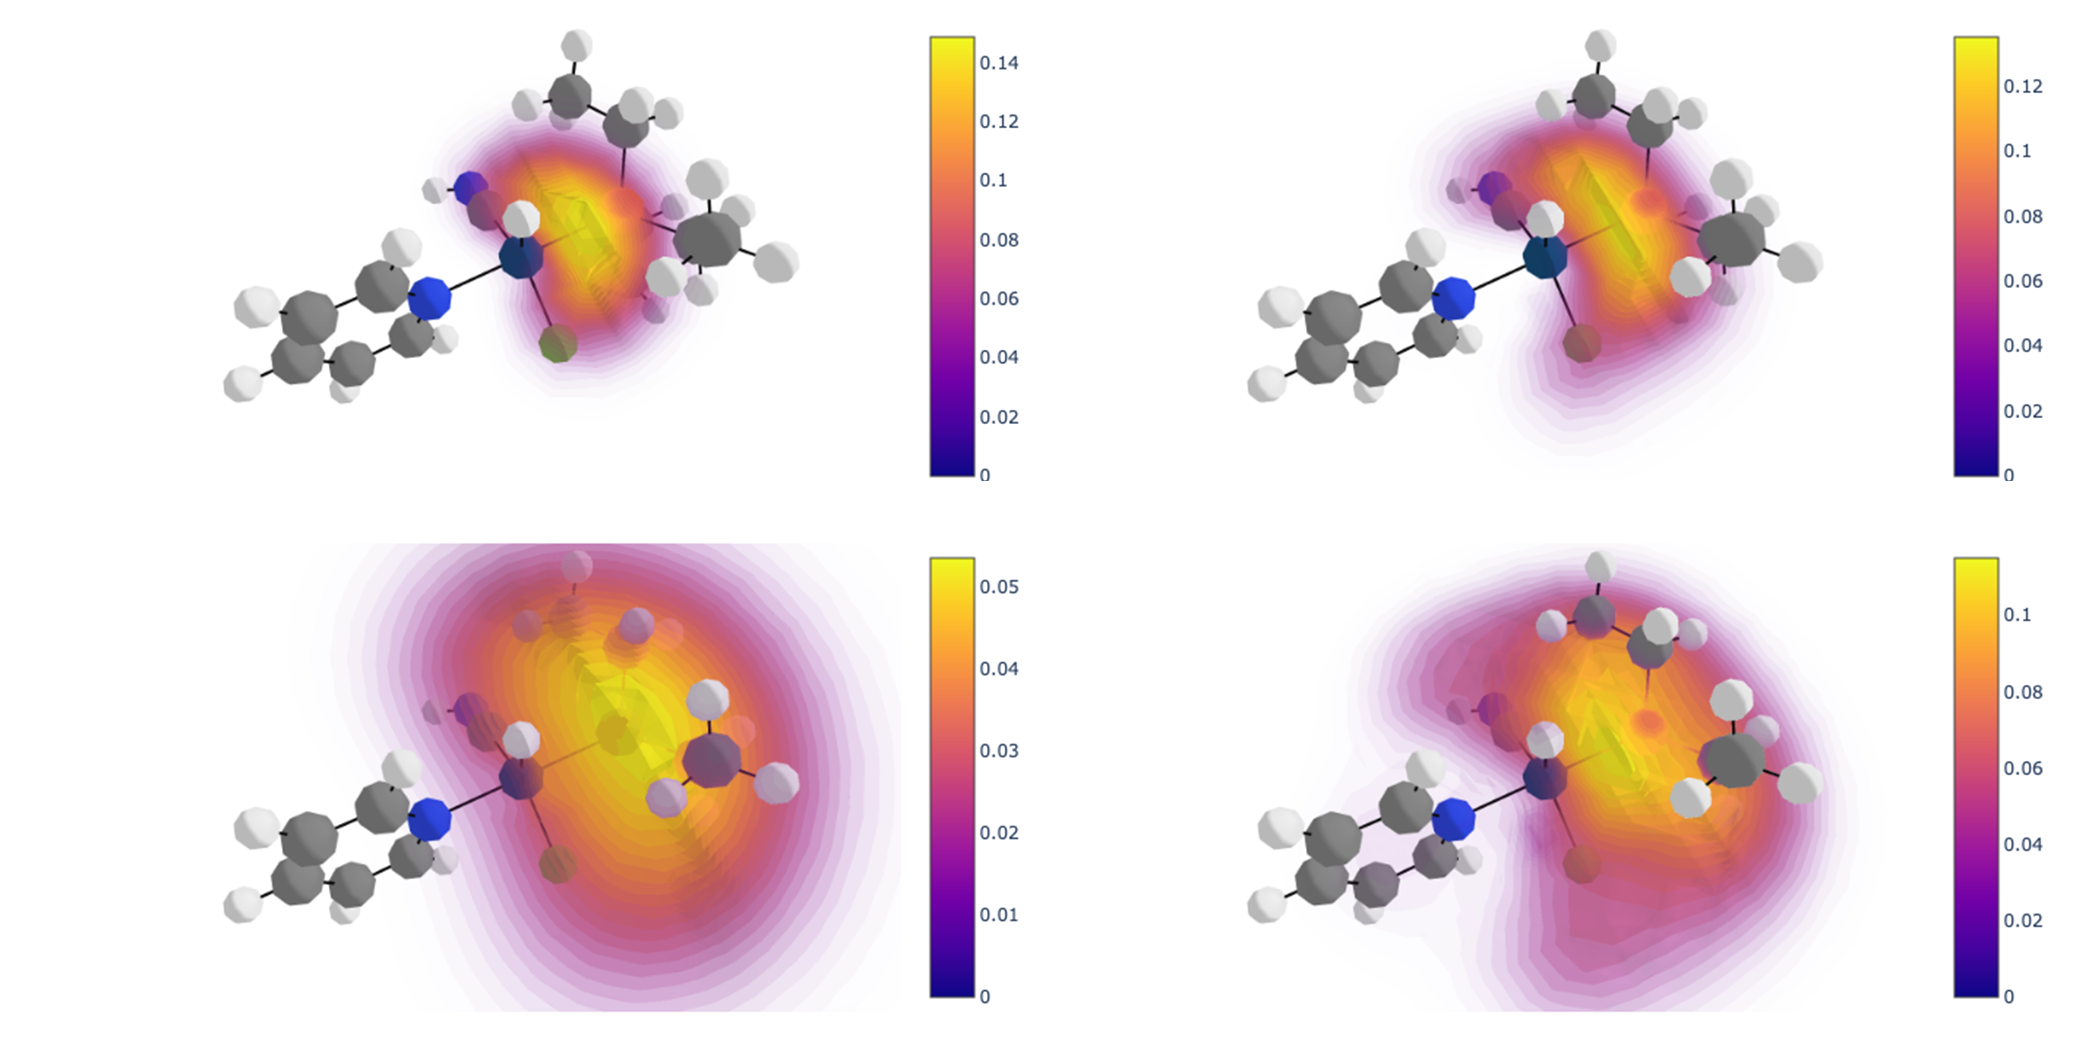
\includegraphics[width=1\textwidth]{figures/snap/density/dense.png} % for .pdf files etc use \includegraphics{test.pdf}
  \caption{Visualization of the density reconstructed from $c_{nlm}^Z$ coefficients for different resolutions.
  Top: $r_{cut} = 10$, bottom: $r_{cut} = 25$, left: $n_{max} = l_{max} = 2$, right: $n_{max} = l_{max} = 8$.
  The density shown is visualizing the density for phosphorus only.
  The phosphorus atom is the orange atom surrounded by the density cloud.
  }
  \label{fig:snap-density}
\end{figure}

This means that in many cases, the center of the encoded density and the center of the atom do not match.
Especially when the element contains many atoms of one species, the descriptor struggles to fully encode the space.

While despite these issues the prediction from SNAP features is still possible with high accuracy, it limits the ability to interpret the results.
When using network explainers in combination with SNAP coefficients, this limited accuracy needs to be kept in mind.
